\section{Design Options for Secure Virtualization Systems}
\label{sec.design}

Providing essential system functionality without exposing privileged code is a
critical challenge in the design of secure systems.
Currently, there are two basic approaches.
One, known as system call interposition (SCI), checks and passes system calls
through to the underlying kernel. The other, which we call ``functionality
re-creation," requires rebuilding system functionality with new code. In this
section, we show that both methods are limited in their ability to
prevent attacks in the kernel.
Using our metric described in Section~\ref{sec.metric},
we then propose a new design scheme named \lip, which accesses only popular
code paths through a very small trusted computer base, and utilizes
functionality re-creation within a secure environment for complex implementations.

\subsection{System Call Interposition (SCI)}
SCI systems~\cite{Janus0:96, Janus:99} filter system calls to mediate requests
from untrusted user code instead of allowing it to go directly to the kernel.
The filter checks a pre-defined security policy to decide which system calls are
allowed to pass to the underlying kernel, and which ones must be stopped.
Figure \ref{fig:design_system_call_interposition} illustrates how
system call interposition works. System administrators have direct access to a policy engine that sets and changes security policies.

\begin{figure}%[h]
\centering
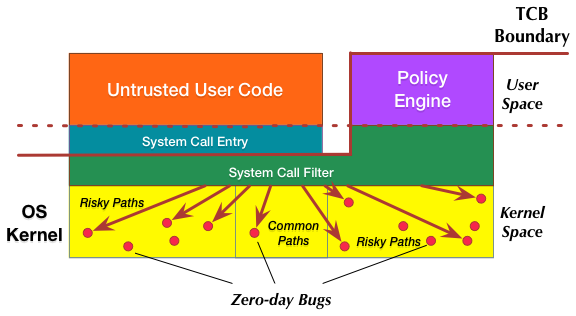
\includegraphics[width=1.0\columnwidth]{diagram/Virtualization_Design_Model_03.png}
\caption{\small Schematic of how System Call Interposition functions.}
\label{fig:design_system_call_interposition}
\end{figure}

SCI was once popular
%approach to the design of secure virtualization systems because
because it gave developers the ability to set and enforce security policies.
%\lois{I think I asked this during the last revision. You say ``was"
%a popular approach. Is it not a popular approach anymore?}
%\yiwen{It is not a popular approach anymore, since no modern design could simply rely on
%this idea to build practical system.}
However, this design is limited by its overly complicated approach to policy
decisions and implementation.
To make a policy decision, the system needs to
obtain and interpret the OS state (e.g., permissions, user groups, register flags)
associated with the programs it is monitoring.
The complexity of OS states makes this process difficult and can lead to
inaccurate policy decisions.
In addition, there are many indirect paths in the kernel that can be accessed.
If security policy makers overlook those paths, it renders the
policy ineffective, as attackers will be able to
bypass security checks.
Moreover, blocking
certain system calls could affect necessary functionality.
It is difficult for developers to fully understand the side-effects of all the
system calls in an interface as complex as the UNIX API.
For example, many applications that rely on \texttt{setuid} fail to check its return value.
If \texttt{setuid} fails, these applications will continue to function in a compromised state,
with incorrect permissions and privileges.
The above limitations make it very challenging to design and build a secure virtualization system using
system call interposition alone.

\subsection{Functionality Re-Creation}
Systems such as Drawbridge \cite{Drawbridge-11},
Bascule \cite{Bascule}, and Graphene \cite{Graphene-14} can
provide richer functionality and run more complex programs than most systems built
with SCI alone because they have their own
interfaces and libraries. We label such a design
as ``functionality re-creation."

\begin{figure}%[h]
\centering
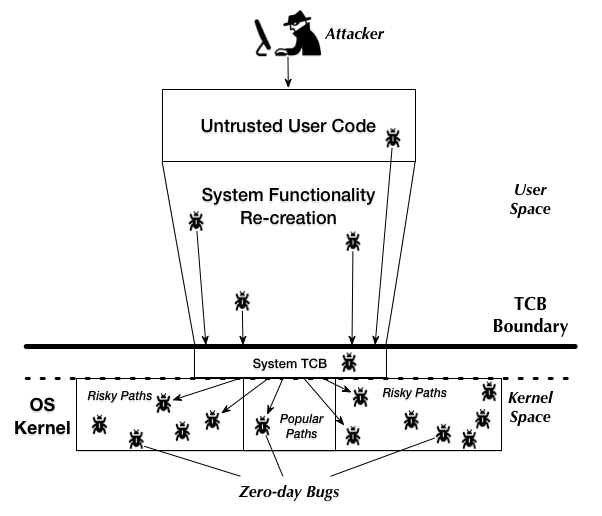
\includegraphics[width=1.0\columnwidth]{diagram/Virtualization_Design_Model_02.png}
\caption{\small Schematic of a Functionality Re-creation System.}
\label{fig:design_functionality_reimplementation}
\end{figure}

The key to this design is to not fully rely on the underlying
kernel for system functions. As illustrated in Figure \ref{fig:design_functionality_reimplementation},
this design re-creates its own system functionalities to provide to user code.
When it has to %communicate with the kernel to
access resources like memory, CPU, and disk storage, the system accesses the kernel directly with
its underlying TCB code.
%which can access the kernel directly.
For example, Graphene \cite{Graphene-14} re-creates
its own Linux system calls in
\texttt{libLinux.so}. When it needs to acquire resources from
the kernel, it uses a
Platform Adaptation Layer (PAL) with access to the kernel,
and provides basic API functions to the OS library.

Functionality re-creation provides a more realistic solution to building
virtualization systems than earlier efforts.
However, hundreds of vulnerabilities have been
reported in existing virtualization systems over the past ten years~\cite{NVD}.
Such systems often
introduce large codebases and enlarged TCBs. In addition, the
complex semantics of OS functions can easily lead to the emergence of bugs during
the re-creation process. Some of these vulnerabilities
can directly cause a privilege escalation, which allows attackers to escape the sandbox
and execute arbitrary code on the host OS.
For example, a vulnerability in VMWare's codebase caused by buffer overflows in the VIX
API allowed local users to
gain privilege to execute arbitrary code in the host
OS, even shellcode to access the kernel of the host OS~\cite{CVE-2008-2100}.


\subsection{Lock-in-Pop: Staying on the Beaten Path }
As discussed above, a weakness of the previous approaches is the inevitable contact
between the privileged kernel code and an untrusted application.
By leveraging our key observation
that ``popular kernel paths contain fewer bugs," we propose a design
in which all code, including the complex part
of the operating system interface, access only
popular kernel paths through a small TCB. As it ``locks" all functionality
requests into only the ``popular" paths, we dubbed the
design \lip.

\begin{figure}%[h]
\centering
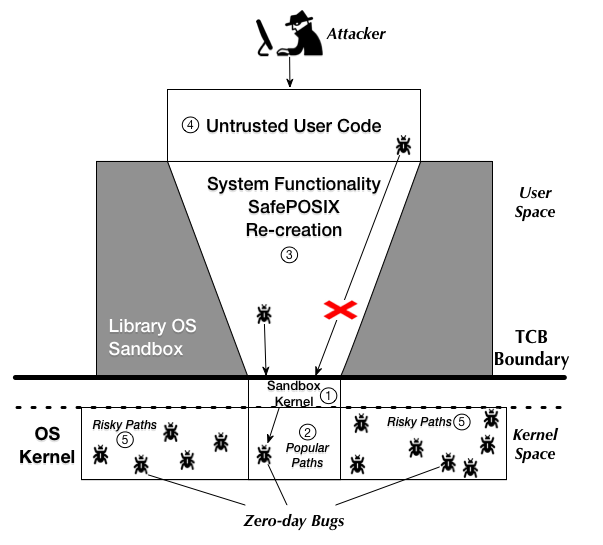
\includegraphics[width=1.0\columnwidth]{diagram/Virtualization_Design_Model_01.png}
\caption{\small \lip system ensures safe execution of untrusted user code
despite existing potential zero-day bugs in the OS kernel.}
\label{fig:design_safe_reimplementation}
\end{figure}

At the lowest level of the design (interfacing with the host OS) is the
sandbox kernel (\ding{172} in Figure \ref{fig:design_safe_reimplementation}).
The sandbox kernel's main role is to ensure that only popular paths (\ding{173} in Figure \ref{fig:design_safe_reimplementation})
of the host OS's kernel can be accessed.
The sandbox kernel could thus function as a very granular system call filter, or
as the core of a programming language sandbox. Note that the functionality
provided by the sandbox kernel is (intentionally) much less than what
an application needs. For example, an application may store files in directories and set permissions on those files.
The sandbox kernel may provide a much simpler abstraction (e.g., a block storage abstraction),
so long as the strictly needed functionality (e.g., persistent storage) is provided.

The application is provided more complex functionality due to the SafePOSIX re-creation
(\ding{174} in Figure \ref{fig:design_safe_reimplementation}).
SafePOSIX has the needed complexity to build the more convenient higher-level
abstractions using the basic functionality the sandbox kernel provides.
The SafePOSIX re-creation is itself isolated within a library OS sandbox, which
forces all system calls from through the sandbox kernel.
So long as this is performed, all calls from SafePOSIX re-creation will only touch the permitted (popular) kernel paths in the underlying host OS.

Similarly, untrusted user code (\ding{175} in Figure \ref{fig:design_safe_reimplementation}) also must be restricted in the way
in which it performs system calls.
System calls must go through the SafePOSIX re-creation, into the sandbox kernel, and then to the host OS.
This is done because if user code could directly make system calls, it could access any paths in the host OS's kernel desired
and thus exploit bugs within them.

Note that it is expected that bugs will occur in many components.
We expect that bugs will occur in the non-popular (risky) kernel paths (\ding{176} in Figure \ref{fig:design_safe_reimplementation}),
bugs will exist in the SafePOSIX re-creation, and the user program will be buggy or even explicitly malicious (created by attackers).
Since the remaining components (\ding{172} and \ding{173} in Figure \ref{fig:design_safe_reimplementation})
are small and/or well tested, this leads to a lower risk of compromise.
